\chapter{Numerical Simulations of Open Quantum Systems}
\thispagestyle{empty}
\label{chap:tech_sec}

This chapter gives a brief introduction to the field of open quantum systems and the Gorini–Kossakowski–Sudarshan–Lindblad (GKSL) master equation, an equation at the heart of simulating Markovian open quantum systems. We introduce numerical algorithms that can be employed to simulate the GKSL master equation more efficiently via stochastic methods. As we will see in the following chapters, the study of open quantum systems does not only lead to a more complete description of quantum systems, but it also leads to the emergence of new phenomena, such as dephasing \cite{pichler2010,sarkar2014} and dissipative phase transitions \cite{diehl2008, carmichael2015, kessler2012, minganti2018}. Furthermore, the loss of information to the environment usually describes an undesirable process; however, it can also be used as a tool to control, in a programable way, the state of a system, giving rise to dissipative state engineering \cite{verstraete2009, muller2012, vidanovic2014}. These effects are not accessible in closed systems, rendering open quantum systems an interesting scenario for exploring new phenomena.

\section{Introduction}

When studying a quantum system, we consider its time evolution governed by some Hamiltonian $\hat{H}$ that describes the dynamics of the system. The most general description of a quantum state is given by its density matrix $\hat{\rho}$ whose evolution can be studied to infer how a system behaves in a given model. Considering a closed quantum system, the von Neumann equation prescribes its time evolution,
\begin{equation}
    \frac{d \hat{\rho}}{dt} = -i \hbar [\hat{H}, \hat{\rho}].
\end{equation}

In the case of a time-independent Hamiltonian (and setting $\hbar =1$), the evolution of the density operator is then given by the equation,

\begin{equation}
    \hat{\rho}(t) = e^{-i \hat{H} t} \hat{\rho}(0) e^{i \hat{H} t}.
\end{equation}

In practice, however, one is usually only interested in a small part of the global system, which can interact with the rest of the system. In order to obtain a description of this smaller subsystem in terms of a Schr\"{o}dinger equation, one would need to neglect the effects of its interactions with its environment and assume it to be a closed system. This, however, is not a realistic description since, often, one cannot simply ignore these interactions.

\begin{figure}[h]
    \centering

    \begin{tikzpicture}
        \node[
            xshift = 0.5cm,
            ellipse,
            draw,fill=blue!20,
            minimum width = 2.5cm,
            minimum height = 1cm,
            label=north: $\hat{H}_{S}$] (sys) at (2,2) {system};
        \node[
            xshift = 7.5cm,
            ellipse,
            draw,
            fill=orange!40,
            minimum width = 5cm,
            minimum height = 2cm,
            label=north: $\hat{H}_{E}$] (env) at (2,2) {Environment};
        \draw[thick,<->] (4.5,2) -- (6,2) node[xshift= -0.7cm,yshift=-0.2cm, anchor=north] {$\gamma$} node[xshift = -0.7cm, yshift = 0.2cm, anchor=south]{$\hat{H}_I$}; 
    \end{tikzpicture}

    \caption{Schematic representation of an open quantum system. The system of interest is coupled to an environment, and the three components describing the overall system are the system Hamiltonian $\hat{H}_S$, the environment Hamiltonian $\hat{H}_E$, and the interaction Hamiltonian $\hat{H}_I$ with coupling rate $\gamma$ between system and environment.}
    \label{fig:Chapter2_Fig1}
\end{figure}

We cannot simply consider the closed system dynamics of the global system, consisting of a system of interest and its environment, due to the exponential scaling of the Hilbert space, which is a difficult problem to solve. This has led to the development of quantum master equations \cite{carmichael1993,breuer2002, manzano2020} to derive equations of motion only for the reduced system (i.e., the system of interest) that account for interactions between the system and its environment but where the environment degrees of freedom have been traced out. Under a set of approximations, which we will discuss later, this leads to a simplified description of only the system of interest, where the effects of the environment on the system are taken into account. 

Without going through the full derivation, we will now introduce the GKSL master equation, perhaps the most well-known master equation, and outline the most important concepts that are at the core of its derivation.

\section{GKSL Master Equation}

As mentioned in the previous section, we will now introduce the GKSL master equation and explain the main ideas behind its derivation. Fig.~\ref{fig:Chapter2_Fig1} shows the schematic representation of the global system $\hat{\rho}_{SE}$ that we are considering; we have the system of interest $\hat{\rho}_S$ with Hamiltonian $\hat{H}_S$, the environment $\hat{\rho}_E$ with Hamiltonian $\hat{H}_E$, and the interaction between system and environment is described by the Hamiltonian $\hat{H}_I$. We combine these components and obtain the global Hamiltonian:
\begin{equation}
    \hat{H} = \hat{H}_S + \hat{H}_E + \hat{H}_I.
\end{equation}

Now, we can write down the time evolution of this global system using the von Neumann equation for density operators, 
\begin{equation}
\label{eq:schr_eq}
    \frac{d}{dt} \hat{\rho}_{SE} = -i [\hat{H}_S+\hat{H}_E+\hat{H}_I, \hat{\rho}_{SE}].
\end{equation}

We then move to the interaction picture by defining the unitary transformations, 
\begin{equation}
\begin{aligned}
    \hat{H}_I(t) = e^{i (\hat{H}_S+\hat{H}_E)t} \hat{H}_I e^{-i (\hat{H}_S+\hat{H}_E)t},\\
    \hat{\rho}_{SE}(t) = e^{i (\hat{H}_S+\hat{H}_E)t} \hat{\rho}_{SE} e^{-i (\hat{H}_S+\hat{H}_E)t},
\end{aligned}
\end{equation}

which allows us to rewrite Eq.~\ref{eq:schr_eq} as:
\begin{equation}
\label{eq:schr_eq_se}
    \frac{d}{dt} \hat{\rho}_{SE}(t) = -i [\hat{H}_I(t), \hat{\rho}_{SE}(t)],
\end{equation}
where we have now introduced the explicit time dependence. As we are interested in the density operator time evolution, we integrate the right-hand side to transform this equation further and obtain, 
\begin{equation}
    \hat{\rho}_{SE}(t) = \hat{\rho}_{SE}(t_0) - i \int_{t_0}^t dt' [\hat{H}_I(t'),\hat{\rho}_{SE}(t')].
\end{equation}

Substituting this expression back into Eq.~\ref{eq:schr_eq_se} we arrive at the following equation, 
\begin{equation}
\label{eq:integro_diff}
    \frac{d}{dt} \hat{\rho}_{SE}(t) = -i [\hat{H}_I(t),\hat{\rho}_{SE}(t_0)] - \int_{t0}^t dt' \big[\hat{H}_I(t), [\hat{H}_I(t'),\hat{\rho}_{SE}(t')]\big]
\end{equation}

As we wish to describe the time evolution of our physical system $\hat{\rho}_S = \Tr_E[\hat{\rho}_{SE}]$, we compute the partial trace over the environment degrees of freedom. Furthermore, we can set the first term to $0$ by choosing an interaction Hamiltonian of the form $\hat{H}_I = \sum\limits_j \hat{S}_j \otimes \hat{E}_j$, where $\hat{S}, \hat{E}$ act on system and environment respectively, and making two assumptions; firstly, that the initial states of the environment and system are not correlated, $\hat{\rho}_{SE}(t_0) = \hat{\rho}_S \otimes\hat{\rho}_E$, and secondly that the initial state of the environment is thermal, $\hat{\rho}_E(t_0) = \exp(- H_E/T)/\Tr[\exp(- H_E/T)]$ with temperature $T$ and setting the Boltzmann constant $k_B=1$. As a result, we can write,
\begin{equation}
\label{eq:integro_diff_trace}
\frac{d}{dt} \hat{\rho}_S(t) = - \int_{t_0}^{t} dt' \Tr_E\big(\big[\hat{H}_ I(t), [\hat{H}_I(t'),\hat{\rho}_{SE}(t')]\big]\big).
\end{equation}
However, having applied the partial trace operator to Eq.~\ref{eq:integro_diff} has not removed the explicit dependence on the global density operator $\hat{\rho}_{SE}$. Furthermore, as it stands now, this expression is exact but very complicated and too difficult to solve analytically or numerically in most cases. For this reason, we will make three approximations, known jointly as the \textit{Born-Markov approximation}, which will allow us to reduce the complexity of this equation heavily. 

\textbf{Born approximation}

The Born approximation assumes that the coupling between the system and environment is weak, which is a valid approximation in many quantum optical systems. The condition is met by simply including all degrees of freedom in the system that strongly interact with each other. Weakly interacting degrees of freedom are kept as the environment. Physically, this means the environment is only minimally affected by interactions with the system, and the system and environment are not entangled. We, therefore, can approximate the total density operator as the tensor product,
\begin{equation}
    \hat{\rho}_{SE}(t) = \hat{\rho}_S(t) \otimes \hat{\rho}_E.
\end{equation}

\textbf{Markov approximation}

The Markov approximation assumes that the time evolution of the system only depends on its current state and has no memory of its past evolution. This means we assume the effects of the interactions between the system and the environment dissipate quickly, and the environment returns back to its equilibrium state to remain approximately static as assumed by the Born approximation. Given the relaxation timescales of the system $\tau_R$ and environment $\tau_E$ for the Markov approximation to hold, we need $\tau_E \ll \tau_R$.

As we have assumed the rapid decay of the environment correlation functions, we can choose $t_0 = 0$ for further simplification and extend the integral from $t$ to $\infty$, which we may do without changing the result.

Applying this together with the \textit{Born-Markov} approximation to Eq.~\ref{eq:integro_diff_trace} we obtain a Markovian master equation, 
\begin{equation}
    \label{eq:born-markov_meq}
\frac{d}{dt} \hat{\rho}_S(t) = - \int_{0}^{\infty} dt' \Tr_E\big(\big[\hat{H}_ I(t), [\hat{H}_I(t'),\hat{\rho}_S(t)\otimes \hat{\rho}_E]\big]\big).
\end{equation}

This equation, also known as the Redfield equation, is trace-preserving but does not guarantee positivity. In order to obtain the GKSL form of the master equation, we need to apply one more approximation, namely the \textit{rotating-wave} approximation. 

\textbf{Rotating-wave approximation}
Let us introduce a general interaction Hamiltonian which can be written in the so-called linear coupling form, 
\begin{align}
    \hat{H}_I(t) &=  \sum_{i,j} \sum_{k}  \Big(\hat{c}_i(t) + \hat{c}^\dagger_i(t)\Big) \Big(\hat{b}_{j,k}(t) + \hat{b}_{j,k}(t)\Big)\\
    &= \sum_{i,j} \sum_{k} (\hat{c}_i(t) \hat{b}_{j,k}(t) + \hat{c}^\dagger_i(t) \hat{b}_{j,k}(t) + \text{h.c.}),
\end{align}
where $\hat{c}_i,\hat{c}^\dagger_i$ denote the system operators, $\hat{b}_{j,k},\hat{b}^\dagger_{j,k}$ denote bosonic environment operators, and h.c. stands for Hermitian conjugate. The index $k$ indicates the sum over the energy modes of the environment, and the Hamiltonian of the environment \cite{gardiner2004} in terms of the bosonic environment operators reads, 
\begin{equation}
    \hat{H}_E = \sum\limits_{j,k} \omega_{j,k} \hat{b}^\dagger_{j,k} \hat{b}_{j,k},
\end{equation}
where $\hat{b}^\dagger_{j,k}, \hat{b}_{j,k}$ satisfiy the bosonic canonical commutation relations.
If we rewrite the operators in the interaction picture, $\hat{c}(t), \hat{b}(t)$ in terms of the Schr\"{o}dinger picture operators $\hat{c}(0), \hat{b}(0)$, we obtain, 
\begin{equation}
\label{eq:int_ham}
    \hat{H}_I(t) = \sum_{i,j} \sum_{k} (\hat{c}_i(0) \hat{b}_{j,k}(0) e^{-i(\omega_i+\omega_{j,k})t} + \hat{c}^\dagger_i(0) \hat{b}_{j,k}(0) e^{-i(\omega_i-\omega_{j,k})t} + \text{h.c.}),
\end{equation}
where $\omega_i, \omega_{j,k}$ are some energy scales of the system and the environment respectively. The rotating wave approximation assumes that these energy scales are approximately equal and we, therefore, obtain two slow-rotating terms $e^{-i(\omega_i-\omega_{j,k})t}$ and two fast-rotating terms, $e^{-i(\omega_i+\omega_{j,k})t}$, and their respective Hermitian conjugates. As the fast-rotating terms oscillate quickly over the typical system relaxation timescale $\tau_R$, they average to zero in this time interval \cite{fujii2017}, and as a consequence, we can omit these terms, which is known as the rotating-wave approximation.
Having described the main approximations used in the derivation of the Markovian master equation, we now present the GKSL form of the master equation, which can be obtained by substituting Eq.~\ref{eq:int_ham} into Eq.~\ref{eq:born-markov_meq}. For the full derivation needed to obtain this form of the master equation, see references \cite{manzano2020}.

\textbf{GKSL master equation}

\begin{equation}
\label{eq:GKSL_meq}
    \dot{\hat{\rho}} = -i [\hat{H}, \hat{\rho}] - \sum_i \frac{\gamma_i}{2} ( \{ \hat{c}^\dagger_i \hat{c}_i, \hat{\rho} \} - 2 \hat{c}_i \hat{\rho} \hat{c}^\dagger_i), 
\end{equation}
where $H$ describes the system Hamiltonian, $\hat{\rho}$ is the system density operator (The subscript \textit{S} has been omitted as we have traced out all environment degrees of freedom, so all operators are now referring to the system.). The operators $\hat{c}_i$ are known as the \textit{Lindblad}, or \textit{jump} operators acting on the $i$-th dissipation channel in a many-body system and describe the type of dissipation that is being simulated in some model of interest. The parameter $\gamma_i$ describes the strength of the dissipation and at what rate energy is being exchanged with the environment. 

We can see from this equation that the first term describes the coherent closed-system time evolution, and the second term describes the resulting dynamics in the system stemming from interactions with the environment, without the need to also simulate the environment and its interactions with the system in a larger Hilbert space. This equation can be solved in many cases for limited system sizes; however, we will now proceed and describe other methods that simulate the GKSL master equation \textit{stochastically}, at the level of the pure vector state instead of the density operator, reducing the dimension of the objects to be simulated, leading to the powerful tool of \textit{quantum trajectories}.

One interesting aspect is that the GKSL Master Equation provides flexibility in choosing jump operators, allowing different sets of related operators to produce the same overall behavior. In contrast, for MIPTs, the choice of operator sets has a clear physical meaning and could lead to different phase transitions. However, even with these differences, the equilibrium state, when averaged over all paths, remains the same.

\section{Quantum Trajectories}

As previously mentioned, we can compute the dynamics of a system coupled to an environment via the GKSL master equation. Numerically, this entails that we need to manipulate and store density operators $\hat{\rho}$, which live in an exponentially large Hilbert space $\mathcal{H}$, represented numerically by matrices consisting of $dim(\mathcal{H})^2$ elements. A pure vector state, however, is numerically represented by a vector consisting of $dim(\mathcal{H})$ elements, which is the motivation behind the so-called \textit{Monte-Carlo} wavefunction method \cite{dum1992, dalibard1992, molmer1993, carmichael1993, plenio1998}, which is a possible choice for the stochastic unraveling of the master equation. This method allows us to simulate the dynamics of the density operator under the GKSL master equation, as in Eq.~\ref{eq:GKSL_meq}, by time-evolving pure states $\{\ket{\psi_i(t)}\}_i$ (with $dim(\mathcal{H}) = 2^M$), sampled from an initial state $\hat{\rho}(t=0)$ and using them to compute individual random trajectories whose statistical averages recover the master equation. Given enough trajectories we can then write $\hat{\rho}(t) = \overline{\ket{\psi(t)}\bra{\psi(t)}}$, where $\overline{\cdot\cdot\cdot}$ denotes the stochastic average over trajectories. This method can be more efficient than the direct simulation of the master equation involving the density operator, as only $dim(\mathcal{H})$ coefficients are required to store a single pure vector state instead of $dim(\mathcal{H})^2$. Still, we must bear in mind that this comes at the cost of having to sample many trajectories to minimize statistical errors, but this is a less restrictive problem as many trajectories can be run in parallel. In the following two sections, we will discuss first-order and higher-order methods, how they are implemented concretely, and how they can be interpreted physically. 

\subsection{First-Order Method}

To obtain a first-order trajectory method, we begin by defining the non-Hermitian effective Hamiltonian,

\begin{equation}
	\label{eq:heff}
	\Heff = \hat{H} - i  \frac{\gamma}{2} \sum\limits_i \hat{c}_i^\dagger \hat{c}_i,
\end{equation}

with which we rewrite the GKSL master equation \ref{eq:GKSL_meq},

\begin{equation}
	\label{eq:meq_heff}
	\dot{\hat{\rho}} = -i [\Heff, \hat{\rho}] + \gamma \sum\limits_i \hat{c}_i \hat{\rho} \hat{c}_i^\dagger.
\end{equation}

To simulate an individual trajectory, we sample a pure state $\ket{\psi{(t =0)}}$ from the initial state $\hat{\rho}(t = 0)$.  With this, we are able to set up an iterative algorithm that computes the dynamics under the effective Hamiltonian undergoing random jumps. The state at time $t+ dt$ in first-order reads,
\begin{equation}
	\label{eq:traj_dt}
	\ket{\psi(t+dt)} = (1 - i \Heff dt) \ket{\psi(t)}.
\end{equation}

As we time evolve under a non-Hermitian effective Hamiltonian, the norm decreases, 
	\begin{align}
    \label{eq:dp}
		\braket{\psi(t+dt)} &= \bra{\psi(t)} (1 + i \Heff^\dagger dt)(1- i \Heff dt)  \ket{\psi(t)} \\
		&= 1 - \gamma dt \sum\limits_i  \bra{\psi(t)} \hat{c}^\dagger_i \hat{c}_i  \ket{\psi(t)} \equiv 1 - \sum\limits_i \delta p_i = 1 - \delta p,
	\end{align}
where the $\delta p_i$ can be seen as the probabilities with which a jump, described by the operator $\hat{c}_i$ will occur in the time interval between $t$ and $t+dt$. 
After propagating the state under the effective Hamiltonian, we make a stochastic selection,
\begin{itemize}
	\item with probability $1-\delta p$, we renormalize the state:
	\begin{equation}
		\ket{\psi(t+dt)} = \frac{	\ket{\psi(t+dt)} }{\sqrt{\delta p}},
	\end{equation}
\item and with probability $\delta p$ a jump occurs:
	\begin{equation}
		\label{eq:jump}
	\ket{\psi(t+dt)} = \frac{	\hat{c}_i \ket{\psi(t)} }{\sqrt{\delta p_i/dt}},
	\end{equation}
where we choose $\hat{c}_i$ randomly according to to the probabilities $\Pi_i = \delta p_i/\delta p$. 
\end{itemize}
This procedure is then repeated to compute the time evolution for a single trajectory until we reach some desired final time $T$.

\begin{mylisting}
    function trajectory(psi0, c, dt, time, Heff)
        psi_t = psi0; % Initialize \psi(t) 
        for t = 1:length(time)-1
            psi_t = (id-1i*dt*Heff)* psi_t; % compute \psi(t+dt) 
            dp = 1-norm(psi_t)^2; % compute jump probability
            if rand < dp 
                % determine where to apply the jump operator
                l = randomJump(psi_t); 
                psi_t = c{l}*psi_t; % apply jump operator
            end
            psi_t = psi_t/norm(psi_t); % renormalize
            % calculate and save observables here
        end
    end
\end{mylisting}    

This pseudocode outlines the described procedure, we have the initial state $\texttt{psi0}$, the array $\texttt{c}$ containing the jump operators $\hat{c}_i$ in position $i$, the numerical time step $\texttt{dt}$, time vector $\texttt{time}$, and the effective Hamiltonian $\texttt{Heff}$. We first initialize a temporary variable containing the initial state and use it in the first time step to compute the state at time $t+dt$ according to Eq.~\ref{eq:traj_dt}. We then compute the jump probability and generate a random number that is uniformly distributed between $0$ and $1$. If it is less than the jump probability we apply a jump operator at a random site $l$. To determine $l$ using $\texttt{randomJump}$, we compute $\Pi_i = \delta p_i/\delta p$ as mentioned above and we define intervals between $0$ and $1$ whose size is proportional to $\delta p_i$. We then draw again a random uniformly distributed number between $0$ and $1$ and pick the index $l$ of the interval in which the random number lies. After this step, we simply renormalize and compute observables or save the state at time $t+dt$ before repeating it until the final simulation time is reached. This has to be then repeated for a large number of trajectories, and upon averaging over many trajectories, we are able to recover the time evolution under the GKSL master equation \ref{eq:GKSL_meq}, which we will prove in the next paragraph.

\textbf{Recovery of the master equation:}

To demonstrate that this stochastic method is equivalent to the master equation \ref{eq:meq_heff} let us consider the density operator of a pure state at a time $t$,
\begin{equation}
 	\hat{\rho}(t) = \ket{\psi(t)} \bra{\psi(t)}.
\end{equation}
As described in the algorithm, with probability $1-\delta p$, we choose the renormalized state, and with probability $\delta p$, we choose the state where a jump occurred. Then, the averaged density matrix at time $t+\delta t$ will be given by the following average,
\begin{equation}
	\overline{\hat{\rho}(t+dt)} = (1-\delta p) \frac{\ket{\psi(t+dt)} \bra{\psi(t+dt)}}{1-\delta p} + \delta p \sum\limits_i \frac{\delta p_i}{\delta p}  \frac{ \hat{c}_i \ket{\psi(t)} \bra{\psi(t)}\hat{c}^\dagger_i}{\delta p_i/dt},
\end{equation}
where $\overline{\hat{\rho}}$ denotes a statistical trajectory average for a given $\hat{\rho}$. With the above definition in equation~\ref{eq:traj_dt} the first term yields: 
\begin{align}
	\ket{\psi(t+dt)} \bra{\psi(t+dt)} &= (1- i dt \Heff ) \ket{\psi(t)} \bra{\psi(t)} (1+ i dt \Heff^\dagger ) \\
	&= (\ket{\psi(t)} - i dt \Heff \ket{\psi(t)} ) (\bra{\psi(t)} - i dt \bra{\psi(t)} \Heff) \\
	&= \hat{\rho}(t) - i dt (\Heff \hat{\rho}(t) - \hat{\rho}(t) \Heff^\dagger),
\end{align}
where in the last line, we omit terms that are not linear in $dt$. 
We obtain: 
\begin{equation}
	\overline{\hat{\rho}(t+dt)} = \hat{\rho}(t) - i dt (\Heff \hat{\rho}(t) - \hat{\rho}(t) \Heff^\dagger)+ dt \sum\limits_i  \hat{c}_i \hat{\rho}(t) \hat{c}^\dagger_i,
\end{equation}
which is equivalent to the Markovian master equation \ref{eq:meq_heff} in a single time step $dt$. Hence we have shown that the algorithm described in this section recovers the evolution under the master equation upon trajectory averaging. 

\subsection{Higher-Order Method}
\label{subsec:higher_order}
In the previous section, we have seen a first-order quantum trajectory method, which time evolves the state using a first-order Taylor expansion of the application of the evolution operator. We can improve the accuracy of this, at the cost of computing a matrix exponential of the effective Hamiltonian, by time evolving via, 
\begin{equation}
	\ket{\psi(t+dt)} = e^{- i \Heff dt} \ket{\psi(t)},
\end{equation}
and then applying the jumps as previously discussed. Computationally, in comparison to before, this step is more costly to perform, as here, the matrix exponential needs to be evaluated. This, however, can be circumvented by using the sparsity of the Hamiltonian or by using functions that compute the action of the exponential operator on the state, see, e.g., Ref.~\cite{expv}. This does not circumvent the fact that jumps require a full time step, leading to an underestimation of the rate at which jumps occur. This can be improved by considering a method that allows the computation of the jump times with arbitrary precision. We start the routine as described in the previous section by sampling a pure state from the initial state $\hat{\rho}(t=0)$. 

We then solve the following equation numerically or analytically for $t_{i+1}$,
\begin{equation}
\label{eq:jumptime}
	||e^{-i \Heff t_{i+1}} \ket{\psi(t_i)} ||^2 = r,
\end{equation}
where $r$ is a uniformly distributed random number between 0 and 1 and $t_{i+1}$ is the time at which the next jump will occur. 
We then compute the time evolution of the state for the time interval $t \in [t_i, t_{i+1}]$ via
\begin{equation}
	\ket{\psi(t)} = \frac{1}{N}  e^{- i \Heff (t -t_i)} \ket{\psi(t_i)},
\end{equation}
with normalization factor: $N = || e^{- i \Heff (t -t_i)} \ket{\psi(t_i)} ||$.

At the time $t = t_{i+1}$, we then apply the quantum jump in the same fashion as described in Eq.~\ref{eq:jump},
	\begin{equation}
	\label{eq:jump_higher}
	\ket{\psi(t_{i+1})} = \frac{	\hat{c}_i \ket{\psi(t_{i+1})} }{\sqrt{\delta p_i/dt}}.
	\end{equation}

As for the first-order method, we repeat these steps to compute the time evolution over the desired time-interval and compute many trajectories over which we compute statistical averages to recover the evolution of the density operator $\hat{\rho}$ under the GKSL master equation \ref{eq:GKSL_meq}. 

Computationally, this method only differs minimally from the previously outlined pseudocode here rather than time evolving with a constant time step throughout the whole simulation, we can numerically solve the exact time at which the jump occurs with arbitrary precision and use any time step we wish, so long as we can accurately compute the state at some time $t$. If, for example, we time evolve a system in the time interval $t\in[0,1]$ using a numerical time step of $dt=0.1$, we have a total of 10 iterations to reach the final simulation time. If at $t=0.35$ a jump occurs, using the first-order method, we will not apply the jump until we reach the time $dt=0.4$. To apply the jump at the exact time it is supposed to occur, we would need to consider a time step of $dt=0.01$, which would require $100$ iterations to reach the final simulation time. Using the higher-order method to compute the jump time exactly and use the numerical time step $dt=0.1$ until we reach the step before the jump, then decrease our time step to the difference between the time when the jump happens and the current time, $dt=0.35-0.3=0.05$. We then apply the jump at this time and continue time-evolving until we reach the final simulation time. This way, we achieve the same accuracy as the first-order method but using only $11$ iterations. When the dissipation rate is low, and jumps only rarely occur, the error tends to remain low, rendering the first-order method a good choice for simulations. When the dissipation rate increases, however, the number of jumps will be underestimated, decreasing the accuracy cumulatively as one time evolves. If, for example, the number of jumps happening in this time interval passes $10$, the average time between jumps will be smaller than the numerical time step, as only $10$ time steps are needed to reach the final simulation time. This simple example demonstrates that as the number of jumps increases with the dissipation rate and the average time between jumps decreases, the first-order becomes increasingly inaccurate due to the over-estimation of when the next jump will occur unless one is willing to reduce the time step significantly. Especially in this regime where the dissipation rate is larger, the higher-order method can prove very useful for both efficiency and accuracy. Note that this has completely ignored the fact that the computation of solving when the jump occurs exactly can also be numerically expensive, so one needs to take into account all these considerations when choosing a method. As we will later show, this computation can also be straightforward to perform, providing both immense improvements in accuracy and computation times.

\subsection{Physical Interpretation}

As we have seen, the quantum trajectory method consists of two parts: the time evolution under an effective Hamiltonian and the random application of jump operators, which simulate the dissipative dynamics of the model. To give some physical context to this method, let us consider a simple two-level system that experiences spontaneous emission \cite{cohen1992}. If we drive the system, we will see coherent Rabi oscillations where the population is transferred back and forth between the ground and the excited state. The Hamiltonian describing this system is given by,
\begin{equation}
    \hat{H} = - \frac{\Omega}{2} (\hat{\sigma}_+ + \hat{\sigma}_-) - \Delta \hat{\sigma}_+ \hat{\sigma}_-,
\end{equation}
where $\Omega$ is the Rabi frequency, characterizing the interaction strength between the system and an external oscillating electromagnetic field, $\Delta$ is the detuning from the resonant frequency, and $\hat{\sigma}_+, \hat{\sigma}_-$ are the raising and lowering operators respectively. The master equation describing the dynamics of the system is given by, 
\begin{equation}
    \dot{\hat{\rho}} = -i [\hat{H}, \hat{\rho}] - \frac{\gamma}{2} \big( \{ \hat{\sigma}_+ \hat{\sigma}_-, \hat{\rho} \} - 2 \hat{\sigma}_- \hat{\rho} \hat{\sigma}_+ \big). 
\end{equation}

\begin{figure}[ht]
    \centering
    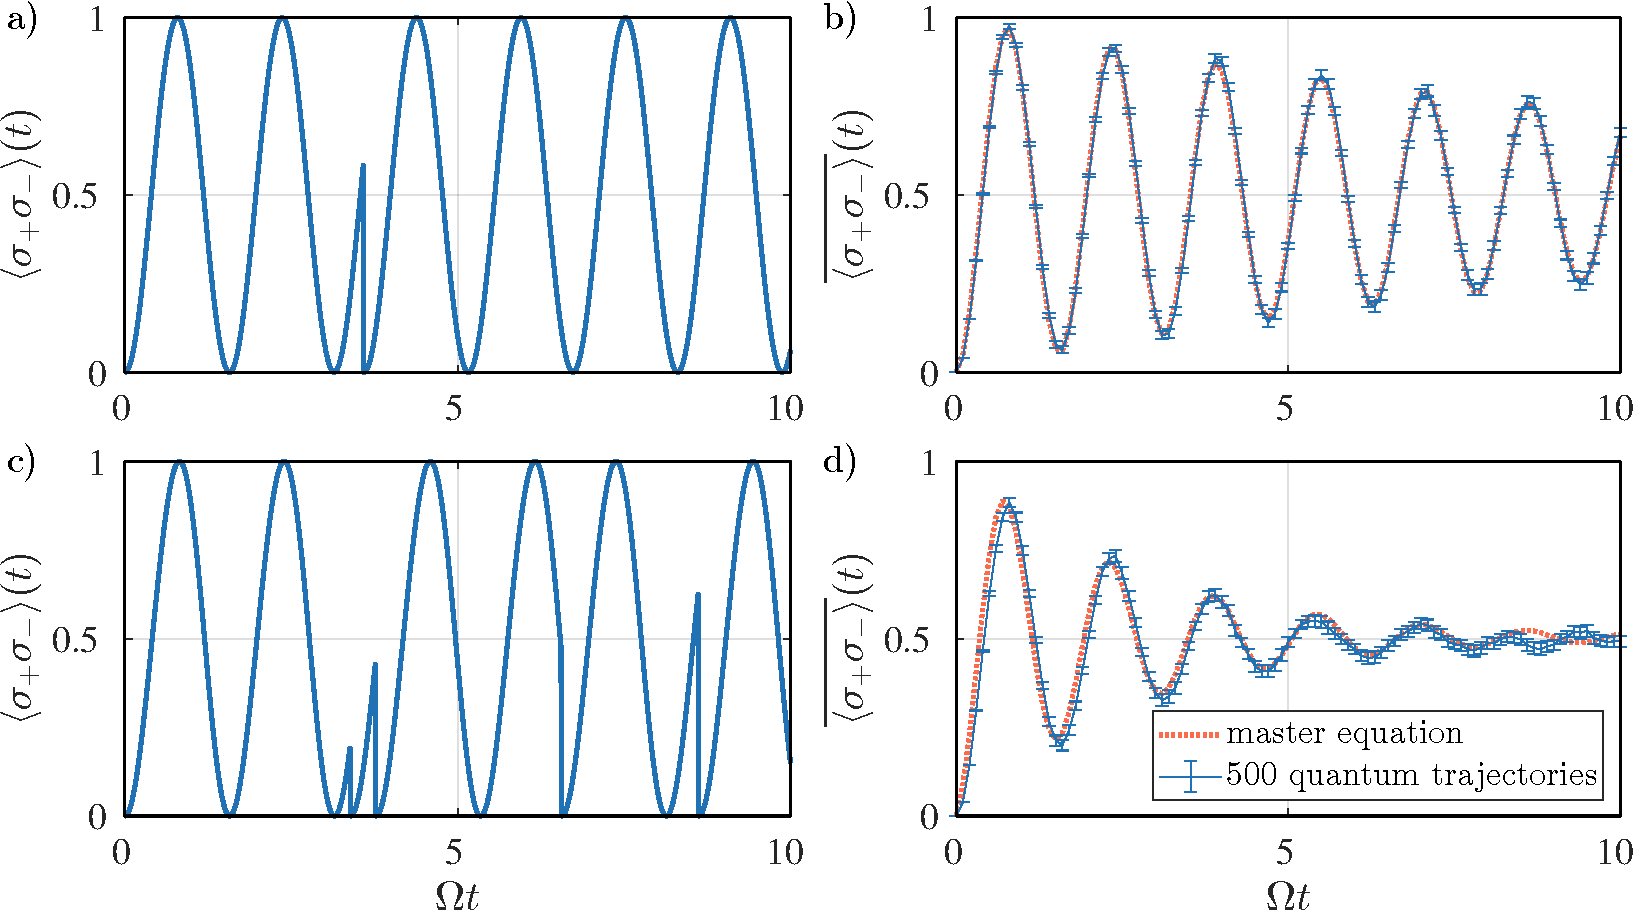
\includegraphics[width=\textwidth]{Chapters/Plots/Chapter3/Chapter2_Fig2.pdf}
    \caption{a), c) Excited state population $\expectation{\hat{\sigma}_+ \hat{\sigma}_-}$ of a two-level system as a function of time in an individual trajectory for two spontaneous decay rates $\gamma = 0.1, 0.5$. Starting from the ground state, the excited state population oscillates coherently at the Rabi frequency $\Omega = 2$ while being interrupted randomly by spontaneous emissions. b), d) Trajectory-averaged excited state population $\overline{\expectation{\hat{\sigma}_+ \hat{\sigma}_-}}$ as a function of time for two spontaneous decay rates $\gamma = 0.1, 0.5$. We compare the quantum trajectory result (blue) to the direct simulation of the master equation (red), where the jump operator is the lowering operator $\hat{\sigma}_-$. We observe good agreement between both methods, using a numerical timestep $dt=10^{-2}$, averaging over $N_t = 500$ trajectories. The statistical errors are computed by dividing the standard deviation of the excited state population by the square root of the number of trajectories \cite{daley2014}.}
    \label{fig:Chapter2_Fig2}
\end{figure}

In Fig.~\ref{fig:Chapter2_Fig2}~a), c) the population of the excited state in a single trajectory is visualized for two spontaneous decay rates $\gamma = 0.1, 0.5$, where the jump operator is the lowering operator $\hat{\sigma}_-$. Starting from the ground state, the system undergoes Rabi oscillations, and we observe the population oscillating between the ground and excited state. Due to spontaneous emission, the atom gets projected into the ground state at random times, and the coherent oscillations are interrupted. With an increasing spontaneous emission rate, we observe the projection into the ground state more frequently. 

In Fig.~\ref{fig:Chapter2_Fig2}~b), d) we display the trajectory-averaged population of the excited state and observe that the quantum trajectory method (blue) recovers the expected dynamics from the master equation (red). An increase in the spontaneous emission rate leads to a stronger damping of the population of the excited state. This example illustrates how individual trajectories can be physically interpreted. The jumps that are randomly applied during the evolution correspond to a sequence of spontaneous emission events that interrupt the coherent dynamics, and if we were to measure the environment, we would gain knowledge that the system was projected into the ground state whenever a photon is detected. In contrast, the time evolution under the effective Hamiltonian corresponds to the coherent dynamics, during which the system undergoes Rabi oscillations. Averaging over many trajectories, we recover the evolution prescribed by the GKSL master equation, where we see the damping effect of the Rabi oscillations caused by spontaneous emissions.

From Fig.~\ref{fig:Chapter2_Fig2}~a), c) we observe at the trajectory level that the number of spontaneous emissions increases with the decay rate. Therefore, the probability of finding the state in the excited state decreases due to an increasing number of projections to the ground state. After some time, $\delta t$, the probability of finding the atom in the excited state is $P_e = \dfrac{\Omega^2 \delta t^2}{4}$. If the decay rate is increased, the number of jumps increases, and the average time $\delta t$ between jumps decreases, and as a consequence, the probability of finding the state in the excited state decreases. This phenomenon, referred to as the \textit{quantum Zeno effect} was first discovered by Itano et al. \cite{itano1990} and is characterized by its tendency to suppress coherent processes, illustrated explicitly in this context by the inhibition of Rabi oscillations. One important point to note is that the equivalence between the Lindblad master equation and the quantum trajectory method is valid for arbitrary decay rates. When increasing the decay rate in numerical simulations, one has to ensure that the numerical parameters are chosen appropriately and that the trajectory-averaged dynamics still coincide with the dynamics resulting from the master equation. Physically, however, the Markov approximation assumes that the environment returns rapidly back to its equilibrium state after being excited, and, therefore, the spontaneous decay rate cannot be increased arbitrarily. At some point, the necessary separation between energy scales is no longer present, and the Markov approximation no longer holds. This means that although the equations themselves do not break, there comes a point where they no longer accurately describe the model that is initially considered.

The unraveling of the master equation we have discussed here is not unique, and in the next section, we will introduce another method, known as \textit{quantum state diffusion} relating to quantum measurement theory. These methods were developed around the same time \cite{gisin1992} as the quantum jump approaches and entail a different physical interpretation, which we will discuss as well. Rather than jump processes that model the dissipative dynamics, a stochastic Schr\"{o}dinger equation approach is used with random noise to model the incoherent dynamics.

\section{Homodyne Detection and Quantum State Diffusion}

As mentioned, the previous quantum jump approach is not a unique unraveling of the master equation, and we can write down other quantum trajectory methods. One such method, known as \textit{quantum state diffusion}, is the result of the analysis of stochastic differential equations and was first derived by \cite{gisin1992,wiseman1993}. We will discuss this further in chapter \ref{chap:MIPT_continuous_measurement} as this method lies at the heart of our work in that chapter. Instead, we will focus on the mathematical background and present the algorithm. We will also put it in the context of \textit{homodyne detection} to have a physical interpretation of this method.

\subsection{Quantum State Diffusion}
\label{subsec:qsd}
The GKSL master equation, Eq.~\ref{eq:GKSL_meq}, can be rewritten as a stochastic differential equation for a pure state $\ket{\psi}$, which is known as \textit{quantum state diffusion}. The following stochastic Schr\"{o}dinger equation (SSE) simulates the dynamics of a single trajectory,

\begin{align}
\label{eq:schr_sse}
\begin{split}
    \ket{\psi(t+dt)} &= \big[ 1 - i \hat{H} - \frac{\gamma}{2} \sum\limits_i \hat{c}^\dagger_i \hat{c}_i \big] \ket{\psi(t)} dt \\ 
&+ \big[ \sum\limits_i \frac{\gamma}{2} \expval{\hat{c}_i+\hat{c}^\dagger_i} \hat{c}_i + \sqrt{\gamma} \hat{c}_i \frac{dW_i(t)}{dt} \big] \ket{\psi(t)} dt,
\end{split}
\end{align}
where $\hat{c}_i,\hat{c}^\dagger_i$ are the jump operators, $dW_i(t)$ is a Wiener increment in It\^o form \cite{wiseman2009} and leads to a noisy output signal, which we further discuss in the next sections. Furthermore, the Wiener increment is not correlated in time or with other sites in the system, which we formally express as, 
\begin{align}
\begin{split}
\label{eq:noise}
        E[dW_i(t)] &= 0 \\
        E[dW_i(t) dW_j(t')] &= dt \delta_{i,j} \delta_{t,t'}.
\end{split}
\end{align}

Note that Eq.~\ref{eq:schr_sse} yields an unnormalized state, so in numerical simulations, one must explicitly normalize in each time step. Furthermore, this equation shows how the time evolution of the state at time $t+dt$ is conditioned on the expectation value of the observable $\expval{\hat{c}_i+\hat{c}^\dagger_i}$ at time $t$. This measurement corresponds to measuring the $x$ quadrature of the system, with the $x$ quadrature operator defined as $\hat{x} = \hat{c}+\hat{c}^\dagger$. This naturally emerges when considering a homodyne detection scheme, which is the topic of the next section. 

\subsection{Homodyne Detection}
\label{subsec:hom_detec}

Homodyne detection is a scheme where an output signal of a system of interest and a local strong oscillator field are mixed in a low-reflectivity beamsplitter (LRBS), as can be seen in Fig.~\ref{fig:Chapter2_Fig3}. The output signal gets recorded by a photodetector and is proportional to the homodyne current $J_\text{hom}$, in which the $x$ quadrature of the system output field is encoded. To see why this is the case, we will provide a brief derivation for the case of \textit{balanced homodyne detection} at the end of this section.

\begin{figure}[ht]
    \centering
    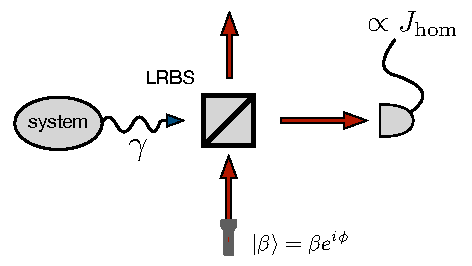
\includegraphics[width=9cm]{Chapters/Plots/Chapter3/Chapter2_Fig3.pdf}
    \caption{A schematic representation of the homodyne detection scheme. The system output signal is mixed in a low reflectivity ($R \to 0$) beamsplitter with a strong local oscillator. The state of the local oscillator is given by $\ket{\beta} = \beta e^{i \phi}$, where $\beta$ is the amplitude and $\phi$ the phase of the oscillator.}
    \label{fig:Chapter2_Fig3}
\end{figure}

Intuitively, we can think of this setup as mixing an unknown signal with a reference signal, allowing us to learn about the unknown system signal, but only weakly probing it and not fully collapsing the system wavefunction. As atoms have the ability to relax through fluorescence, they can emit photons into their electromagnetic environment. In experiments through detecting and counting the emitted photons, discrete quantum jumps of the state can be observed, collapsing the system wavefunction as we saw in the previous section. If, instead, the amplitude of the fluorescence field is mixed coherently with a local oscillator by a beamsplitter, then each realization of a measurement record can be used to construct a quantum trajectory whose evolution obeys quantum state diffusion, and a homodyne current can be measured. This is related to chapter \ref{chap:MIPT_continuous_measurement} where we consider a system of free fermions and use the homodyne current that arises in such a setup to investigate the measurement-induced phase transition that arises in this model. As we will discuss later, the local oscillator also amplifies the system output signal, so this setup is also useful when the output from the system is weak.

In this setup, only the transmitted signal is recorded in a photodetector, and although a low-reflectivity beamsplitter is used, some of the system signal will be reflected and lost. To counteract this, the local oscillator $\beta$ amplitude must be large. To completely avoid the loss of signal, we need the reflectivity $R$ of the beamsplitter to go to zero ($R \to 0$), which in turn means the amplitude $\beta$ of the local oscillator needs to be infinite ($\beta \to \infty$). In this limit, the photodetection rate goes to infinity, but as the local oscillator dominates the recorded signal, the effect on the system goes to zero. This means the collapses that the system experiences due to the measurement process become infinitesimally small; however, they happen at an infinite rate, leading to a continuous evolution in time of the conditioned state of the system. As individual collapses only affect the state of the system infinitesimally, the photocurrent at the detector needs to be integrated over a time interval $\Delta T$, chosen such that $\Delta T$ is small compared to times over which the system changes significantly, but large enough to have witnessed a large number of collapses. This treatment leads us to the approach of describing this setup using a stochastic Schr\"{o}dinger equation (SSE) (Eq.~\ref{eq:schr_sse}), and full derivations of this can be found in Refs.~\cite{carmichael1993}.

\textbf{Balanced Homodyne Detection}
Homodyne detection has proven to be a useful setup for measuring the dynamics of a system state that is conditioned on its measurements. Balanced homodyne detection (BHD) works similarly, and its setup is shown schematically in Fig.~\ref{fig:Chapter2_Fig4}.

\begin{figure}[ht]
    \centering
    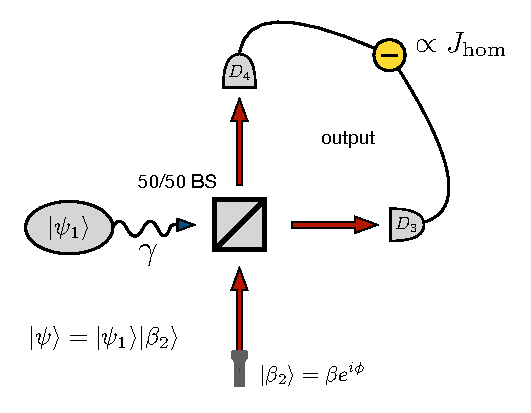
\includegraphics[width=9cm]{Chapters/Plots/Chapter3/Chapter2_Fig4.pdf}
    \caption{The homodyne detection setup consists of a $50/50$ beamsplitter, which mixes the system output equally with a strong local oscillator. The two output beams are then subtracted, and the resulting signal is proportional to the homodyne current $J_\text{hom}$.}
    \label{fig:Chapter2_Fig4}
\end{figure}

Instead of using an LRBS, a $50/50$ beamsplitter is used instead. The two equally mixed output signals are recorded in photodetectors and subtracted from one another, yielding the output signal. Due to the subtraction of the two signals, noise and fluctuations arising in this setup are canceled out as they often originate from the same source, resulting in BHD being the preferred setup. 

In order to find an expression for the current, let us consider some pure system state $\ket{\psi}_1$, and the local oscillator to be simply a coherent state $\ket{\beta}_2 = \beta e^{i \phi}$. The joint input state then is $\ket{\psi}_\text{in} = \ket{\psi}_1 \ket{\beta}_2$. The photocurrents that are measured on detectors $D_3, D_4$ will be proportional to the expectation value of the respective number operators $\hat{n}_i = \hat{c}^\dagger_i \hat{c}_i$ ($i = 3,4$), where $\hat{c}^\dagger_i, \hat{c}_i$ are the respective raising and lowering operators. We consider a $50/50$ beamsplitter so we have transmittivity $T = \frac{1}{\sqrt{2}}$ and reflectivity $R = \frac{1}{\sqrt{2}}i$ and with this we can rewrite the operators as $\hat{c}_3 = T \hat{c}_1 + R \hat{c}_2$ and $\hat{c}_4 = R \hat{c}_1 + T \hat{c}_2$. 
With some algebra, we can express the difference $\hat{n}_3-\hat{n}_4$ as, 
\begin{align*}
    \hat{n}_3 - \hat{n}_4 &= \hat{c}^\dagger_3 \hat{c}_3 - \hat{c}^\dagger_4 \hat{c}_4   \\
    &= \frac{1}{2} \big[ (\hat{c}^\dagger_1 - i \hat{c}^\dagger_2)(\hat{c}_1 + i\hat{c}_2) - (\hat{c}^\dagger_2 - i \hat{c}^\dagger_1)(\hat{c}_2 + i \hat{c}_1) \big]\\
    &= 2 \big[\frac{1}{2i} (\hat{c}_1 \hat{c}^\dagger_2 - \hat{c}^\dagger_1 \hat{c}_2) \big]. 
\end{align*}
The photocurrent $i_{34} = i_3-i_4$ is proportional to the expectation value of this operator, 
\begin{align*}
    i_3-i_4 & \propto \expval{\hat{n}_3 - \hat{n}_4} \\
    & \propto 2 \bra{\psi} \big[\frac{1}{2i} (\hat{c}_1 \hat{c}^\dagger_2 - \hat{c}^\dagger_1 \hat{c}_2) \big] \ket{\psi} \\
    & \propto 2 \bra{\psi_1} \big[\frac{1}{2i} (\hat{c}_1 \bra{\beta_2}\hat{c}^\dagger_2\ket{\beta_2} - \hat{c}^\dagger_1 \bra{\beta_2}\hat{c}_2\ket{\beta_2}) \big] \ket{\psi_1} \\
    & \propto 2 |\beta| \bra{\psi_1} \big[\frac{1}{2i} (\hat{c}_1 e^{-i \phi} - \hat{c}^\dagger_1 e^{i \phi}) \big] \ket{\psi_1}\\
    & \propto 2 |\beta| \expval{\hat{x}_\phi}_1,
\end{align*}
where $\hat{x}_\phi$ is the generalized quadrature operator. Choosing $\phi = \frac{\pi}{2}$, for example, leads to measuring the $\hat{x}$ quadrature of the system. This simple calculation shows that the subtraction of the two photocurrents leads to a signal that is proportional to the oscillator field amplitude and the measurement of the $\hat{x}$ quadrature of the system for some phase angle $\phi$ of the local oscillator field. BHD leads to the same SSE as in the case of simple homodyne detection, as can be seen in Ref.~\cite{carmichael1993}. To see where the stochastic nature arises from, we can consider a time interval during which the system experiences some number of collapses. These collapses occur randomly in time and can be modelled with a stochastic process. This is why the white noise term appears in the conditioned time evolution of the state. As we consider the limit where the amplitude of the local oscillator goes to infinity ($\beta \to \infty$), the homodyne current becomes a continuous function in time rather than a jump process. The homodyne current is not simply the amplitude of the output signal that we mix with the local oscillator, and it also consists of a white noise term. We define the homodyne current as, 
\begin{equation}
\label{eq:Jhom}
    J_\text{hom} = \frac{\expval{\hat{x}}}{2} + \frac{dW}{\sqrt{\gamma} dt}.
\end{equation}
With this definition we can rewrite the SSE \ref{eq:schr_sse} as, 
\begin{align}
\label{eq:schr_sse_hom}
\begin{split}
    \ket{\psi(t+dt)} &= \big[ 1 - i \hat{H} - \frac{\gamma}{2} \sum\limits_i \hat{c}^\dagger_i \hat{c}_i + \gamma \sum\limits_i J_\text{hom} \hat{c}_i \big] \ket{\psi(t)} dt,
\end{split}
\end{align}
where $J_\text{hom}$ is the current associated to the $\hat{x}$ quadrature operator $\hat{x}_i$. The signal that is picked up by the photodetector is proportional to this homodyne current, and as the white noise term has zero mean, upon averaging over many trajectories, the $\hat{x}$ quadrature of the system output field can be measured. This algorithm is easily implementable and has allowed us to obtain the results presented in chapter~\ref{chap:MIPT_continuous_measurement}.

\section{Fermionic Gaussian States}
\label{sec:FGS}

To conclude our introduction to the numerical tools used in this thesis, we now discuss Fermionic Gaussian States (FGS). These states are fully characterized by their correlation matrix, which we introduce below, substantially simplifying calculations. As mentioned earlier, the density operator that numerically represents a quantum state lives in an exponentially large Hilbert space $\mathcal{H}$. Therefore, it follows that the number of elements needed to store the state numerically also scales exponentially with the number of lattice sites. In contrast, as FGS are completely characterized by their correlation matrix, the number of elements needed for its representation scales with the square of the lattice size. For the simulation of dynamics, FGS have the useful property that they remain Gaussian under time evolution with a quadratic Hamiltonian. This means that the Hamiltonian can only contain quadratic terms in the fermionic raising and lowering operators, which restricts the models we can simulate with them. This section mainly introduces two trajectory algorithms we use to generate the data for chapters~\ref{chap:MIPT_bosons} and \ref{chap:MIPT_continuous_measurement}. The algorithms and methods below are adapted from the following References~\cite{alberton2021,cao2019,surace2022}. 

\subsection{Time evolution with FGS}
For a general Fermionic Quadratic Hamiltonian we write,
\begin{equation}
    \hat{H} = \sum\limits_{i,j} \big(A_{ij} \hat{c}_i^\dagger \hat{c}_j + B_{ij} \hat{c}_i \hat{c}_j \big) + h.c.,
\end{equation}
where $\hat{c}_i^\dagger,\hat{c}_i$ are the fermionic raising and lowering operators acting on site $i$. In this thesis, we only consider number-conserving quadratic Hamiltonians, i.e., $B_{ij} = 0 ~\forall i,j$. $A$ is the hopping matrix and encodes the connections between lattice sites. We parameterize the normalized FGS as follows, 
\begin{equation}
\label{eq:fgs}
\ket{\psi_t} = \prod_{n=1}^N\Big( \sum\limits_{i=1}^M \hat{U}_{i,n}(t) \hat{c}^\dagger_i \Big) \ket{0},
\end{equation}
where $M$ is the number of lattice sites, $N$ is the particle number, and $\hat{U}$ satisfies $\hat{U}^\dagger \hat{U} = \mathbb{I}$. From this parameterization, we compute the correlation matrix, which fully characterizes the FGS,
\begin{equation}
    D_{ij}(t) = \expectation{\hat{c}_i^\dagger \hat{c}_j} = [\hat{U}(t) \hat{U}^\dagger(t)]_{j,i},
\end{equation}
where $\hat{c}_i^\dagger,\hat{c}_i$ are the fermionic raising and lowering operators acting on site $i$. 
Then, the closed system time evolution follows the equation, 
\begin{equation}
\label{eq:timeev}
\hat{U}(t+dt) = e^{-iA dt} \hat{U}(t),
\end{equation}
where $D(t) = [\hat{U}(t)\hat{U}^\dagger(t)]^T$ is the correlation matrix at time $t$, $A$ is the hopping matrix, and $dt$ is the numerical time step.

Finally, for a subsystem $M = [m_i,m_j]$ we can compute the reduced correlation matrix $D_M(t) = D_{m_i,m_j\in M}(t)$. The von Neumann entropy can be computed \cite{surace2022} using,
\begin{equation}
\label{eq:vnE}
S(D_M) = -\sum\limits_{i} \lambda_i \ln\lambda_i + (1-\lambda_i)\ln(1-\lambda_i),
\end{equation}
where $\{\lambda_i\}$ is the spectrum of $D_M$. 

Because FGS are fully characterized by their correlation matrix, we only require $M^2$ to describe a system consisting of $M$ sites fully. Furthermore, as we are also able to calculate the entropy from the correlation matrix, we have efficient methods that we use throughout chapters \ref{chap:MIPT_bosons} and \ref{chap:MIPT_continuous_measurement}.

\subsection{Quantum Jump Algorithm}

To implement the quantum jump algorithm outlined in section \ref{subsec:higher_order}, we use the fact that we are dealing with a number-conserving Hamiltonian, which allows us to compute the times at which quantum jumps occur explicitly. Normally, we would need to solve Eq.~\ref{eq:jumptime} numerically; however, given the total particle number, we can solve this equation explicitly, and the jump times can be computed using, 
\begin{equation}
    t_{i} = t_{i-1} - \frac{\ln{r}}{\gamma N},
\end{equation}
where $t_{i-1}$ is the time when the last jump occurred ($t_0 = 0$), and $r$ is a random number between $0$ and $1$ drawn from a uniform distribution.

We then compute the time evolution of the correlation matrix using Eq.~\ref{eq:timeev} until the first jump occurs. Then, the jump is applied via, 
\begin{equation}
  D_{ij} =
    \begin{cases}
      1, & i = j = k\\
      0, & i \neq j \text{ and } (i = k \text{ or } j = k)\\
      D_{ij} - \frac{D_{kj}D_{ik}}{\expectation{n_k}_t}, & \text{otherwise},
    \end{cases}       
\end{equation}
where $\expectation{n_k}_t$ is the jump operator at site $k$ that has been selected considering the probabilities $p_i$ in Eq.~\ref{eq:dp}. Then, we perform a singular value decomposition, $D = U S U^\dagger$, to obtain a new $U$ matrix, continue time evolving until the next jump, and repeat this process until the end of the simulation.

\subsection{Quantum State Diffusion}

We previously introduced QSD in section~\ref{subsec:qsd}, which we can also simulate efficiently using FGS. This algorithm is generally more efficient as the whole time evolution can be simulated using only the $U$ matrix. We aim to simulate the following stochastic Schr\"{o}dinger equation,
\begin{equation}
\label{eq:SSE}
       \ket{\psi(t+dt} = \Big(1-iH dt + \sum\limits_{i=1}^M\Big[ \sqrt{\gamma} (n_i-\langle n_i\rangle_t) dW_{i,t}- \frac{\gamma}{2} (n_i-\langle n_i\rangle_t)^2 dt\Big]  \Big) \ket{\psi_t},
\end{equation}
which explicitly depends on the expectation value of $n_i(t)$. Note that this expression is equivalent to Eq.~\ref{eq:schr_sse}; however, this equation contains additional normalization terms. Furthermore, the monitored quadrature operator is the local number operator $\hat{c}_i = \hat{n}_i$.  

The time evolution for FGS is implemented using,
\begin{equation}
\label{eq:evol}
U(t+dt) = W e^{-iAdt} U(t),
\end{equation}
where  $W$ is the stochastic matrix $W = \text{diag}(e^{dW_{i,t}+\gamma(2\langle n_i \rangle-1)dt})$, and $A$ is the hopping matrix of the Hamiltonian, $\hat{H} = \sum\limits_{i,j} h_{ij} \hat{c}_i^\dagger \hat{c}_j  + \text{h.c.}$. Here, the factor $\sqrt{\gamma}$ has been absorbed in the white noise term, which now satisfies $E[dW_{i,t}] = 0$ and $E[dW_{i,t}dW_{j,t'}] = \delta_{i,j}\delta(t-t') \gamma dt$. Finally, the normalization of U is enforced via a QR decomposition, $U = QR$, and then redefining $U = Q$, which ensures that $U$ is orthonormal. Then, as with other trajectory algorithms we have discussed, we repeat this process until the final simulation time is reached. 

\section{Summary}

In this chapter, we have introduced the GKSL master equation, which can be used to simulate Markovian open quantum systems. We provided an overview of the derivation and the approximations used to obtain the final form of the equation. We then introduced stochastic unraveling methods of the master equation, namely quantum trajectories, where in individual trajectories, coherent dynamics are interrupted by so-called quantum jumps and quantum state diffusion, where the dynamics of a pure state are governed by a stochastic Schr\"{o}dinger equation. Lastly, we introduce Fermionic Gaussian States (FGS) as a numerical tool to simulate specific models. Specifically, in chapter~\ref{chap:MIPT_bosons}, we use both quantum jump trajectories and quantum state diffusion in combination with FGS to access larger system sizes; in chapter~\ref{chap:MIPT_continuous_measurement}, we use quantum state diffusion and FGS, and lastly, in chapter~\ref{chap:short_time_dynamics} we consider only quantum jump trajectories for limited system sizes.